% =========================================================
% KHAI BÁO CẤU HÌNH (PREAMBLE) - ĐÃ FIX THƯ VIỆN
% =========================================================
\documentclass[aspectratio=169, 9pt]{beamer}

% Load theme HUST
\usetheme[theme=blue,logo=logowithtextvi]{HUST} 

% Các package cần thiết
\usepackage[T5]{fontenc} 
\usepackage[utf8]{inputenc}
\usepackage{lmodern}      
\usepackage{enumitem}     
\usepackage{tcolorbox}    
\usepackage{listings}     
\usepackage{verbatim}
\usepackage{amsmath}
\usepackage[table]{xcolor}
\usepackage{tikz}

\usepackage{minted} 
\usemintedstyle{colorful}
\tcbuselibrary{listingsutf8, skins, minted}

\usetikzlibrary{decorations.pathreplacing,arrows.meta,shapes}

% Định nghĩa lệnh đặt nội dung tự do
\newcommand{\placecontent}[4]{%
  \tikz[remember picture,overlay]
    \node[anchor=north west]
      at ([xshift=#1,yshift=-#2]current page.north west)
      {\parbox{#3}{#4}};
}

% Thông tin metadata
\title{LẬP TRÌNH C CƠ BẢN}
\author{SoICT - HUST}
\date{}

% Chỉnh footer hiện số trang
\setbeamertemplate{footline}{%
  \hfill%
  \insertframenumber\hspace{0.5cm}\vspace{0.3cm}
}

% =========================================================
% NỘI DUNG CHÍNH (BODY)
% =========================================================
\begin{document}

% --- SLIDE 1: TRANG BÌA ---
\HUSTInsertBrandSlide

% --- SLIDE 3 (PDF Page 3): TITLE SLIDE ---
{
\HUSTUseBackground{onelove.pdf}
\begin{frame}
    % Logo góc
    \HUSTCornerImage{assets/logo/04.pdf}

    % Tên môn học
    \placecontent{0.5cm}{0.33\paperheight}{0.85\paperwidth}{
        \color{\HUSTFrameTitleTextColor}\bfseries\fontsize{26pt}{30pt}\selectfont
        C BASIC
    }
    
    % Tên bài học
    \placecontent{0.5cm}{0.50\paperheight}{0.6\paperwidth}{
        \color{\HUSTFrameTitleTextColor}\bfseries\fontsize{17pt}{32pt}\selectfont
        ĐỆ QUY
    }
\end{frame}
}

% --- SLIDE 4 (PDF Page 4): NỘI DUNG ---
\begin{frame}{NỘI DUNG}
    \small
    \begin{itemize}[label=$\bullet$, itemsep=0.8em]
        \item \textbf{Đệ quy}
        \begin{itemize}[label=$\circ$, itemsep=0.4em]
            \item Bài toán ước số chung lớn nhất (P.02.04.01)
            \item Bài toán đổi số nguyên sang chuỗi bít nhị phân (P.02.04.02)
            \item Bài toán tháp Hà Nội (P.02.04.03)
        \end{itemize}
        
        \item \textbf{Đệ quy có nhớ}
        \begin{itemize}[label=$\circ$, itemsep=0.4em]
            \item Bài toán tính dãy số Fibonacci (P.02.04.04) 
            \item Bài toán tính hằng số tổ hợp (P.02.04.05) 
        \end{itemize}
    \end{itemize}
\end{frame}

% --- SLIDE 5 (FIXED): ĐỆ QUY (2x2 Trắng sạch sẽ) ---
\begin{frame}{ĐỆ QUY}
    \small
    \begin{itemize}
        \item \textbf{Định nghĩa:} Đối tượng có cấu trúc đệ quy là đối tượng được định nghĩa/xây dựng qua chính nó với quy mô nhỏ hơn
        \item \textbf{Hàm đệ quy:} là hàm đưa ra lời gọi đến chính nó với quy mô tham số nhỏ hơn
        \item \textbf{Thuật toán đệ quy (thường được thể hiện bởi 1 hàm đệ quy):} phù hợp để thực hiện các xử lý, tính toán trên các đối tượng có cấu trúc đệ quy.
    \end{itemize}

    \vspace{0.1cm}
    \begin{columns}[t]
        \begin{column}{0.49\textwidth}
            \begin{tcolorbox}[colback=white, colframe=blue!60, title=\textbf{Tổng lũy tiến}, left=1pt, right=1pt, fonttitle=\bfseries]
                $$\small F(n) = \begin{cases} F(n-1) + n & n \ge 2 \\ 1 & n = 1 \end{cases}$$
            \end{tcolorbox}
            \begin{tcolorbox}[colback=white, colframe=blue!60, title=\textbf{Ước số chung (GCD)}, left=1pt, right=1pt, fonttitle=\bfseries]
                $$\small F(a,b) = \begin{cases} a & a = b \\ F(a-b, b) & a > b \\ F(a, b-a) & a < b \end{cases}$$
            \end{tcolorbox}
        \end{column}
        
        \begin{column}{0.49\textwidth}
            \begin{tcolorbox}[colback=white, colframe=red!60, title=\textbf{Dãy Fibonacci}, left=1pt, right=1pt, fonttitle=\bfseries]
                $$\small F(n) = \begin{cases} F(n-1) + F(n-2) & n \ge 2 \\ n & n = 0, 1 \end{cases}$$
            \end{tcolorbox}
            \begin{tcolorbox}[colback=white, colframe=red!60, title=\textbf{Hằng số tổ hợp}, left=1pt, right=1pt, fonttitle=\bfseries]
                % Chỉnh lại case để k=0, n không bị tràn
                $$\small C(k, n) = \begin{cases} 1 & k = 0, n \\ C_{k,n-1} + C_{k-1,n-1} & \text{ngược lại} \end{cases}$$
            \end{tcolorbox}
        \end{column}
    \end{columns}
\end{frame}

% --- SLIDE 6 (FIXED): BÀI TOÁN USCLN ---
% Chuẩn theo ảnh image_eb19af.png
\begin{frame}{BÀI TOÁN ƯỚC SỐ CHUNG LỚN NHẤT (P.02.04.01)}
    \small
    \begin{itemize}[label=$\bullet$, itemsep=0.8em]
        \item Cho hai số nguyên dương a và b. Hãy viết chương trình tìm ước số chung lớn nhất của a và b.
        \item Dữ liệu
        \begin{itemize}[label=$\bullet$]
            \item Dòng 1: ghi 2 số nguyên dương a và b ($1 \le a, b \le 100000$)
        \end{itemize}
        \item Kết quả
        \begin{itemize}[label=$\bullet$]
            \item Ghi ra ước số chung lớn nhất của a và b
        \end{itemize}
    \end{itemize}

    \vspace{0.5cm}

    \begin{center}
        \renewcommand{\arraystretch}{1.2}
        \begin{tabular}{|p{4cm}|p{4cm}|}
            \hline
            \centering \textbf{stdin} & \centering \textbf{stdout} \tabularnewline \hline
            16 24 & 8 \tabularnewline \hline
        \end{tabular}
    \end{center}
\end{frame}


% --- SLIDE 7: USCLN MÃ GIẢ ---
\begin{frame}[fragile]{BÀI TOÁN ƯỚC SỐ CHUNG LỚN NHẤT – MÃ GIẢ}
    \begin{columns}[T]
        \begin{column}{0.48\textwidth}
            \vspace{0.4cm}
            \begin{itemize}[label=\textcolor{red!70!black}{$\blacktriangleright$}, itemsep=1.5em]
                \item Nếu $a = b$: \\ \quad $USCLN(a, b) = a$
                \item Nếu $a > b$: \\ \quad $USCLN(a, b) = USCLN(a - b, b)$
                \item Nếu $a < b$: \\ \quad $USCLN(a, b) = USCLN(a, b - a)$
            \end{itemize}
        \end{column}

        \begin{column}{0.48\textwidth}
            \begin{tcblisting}{
                colback=white, colframe=black, boxrule=0.8pt, arc=0pt,
                listing engine=minted, minted language=c,
                minted options={fontsize=\small, autogobble, baselinestretch=1, style=colorful},
                listing only, left=2mm, top=2mm, bottom=2mm
            }
F(a, b) {
    if (a == b) return a;
    if (a > b) return F(a - b, b);
    else return F(a, b - a);
}
            \end{tcblisting}
        \end{column}
    \end{columns}
\end{frame}

% --- SLIDE 8: USCLN CODE ---
\begin{frame}[fragile]{BÀI TOÁN ƯỚC SỐ CHUNG LỚN NHẤT – CODE HOÀN CHỈNH}
    \begin{tcblisting}{
        colback=white, 
        colframe=black, 
        boxrule=0.8pt, 
        arc=0pt, 
        listing engine=minted, 
        minted language=c,
        minted options={
            fontsize=\small, 
            breaklines, 
            autogobble, 
            baselinestretch=1, 
            tabsize=4,
            style=colorful
        },
        listing only,
        left=2mm, top=2mm, bottom=2mm
    }
#include <stdio.h>

int F(int a, int b) {
    if (a == b) return a;
    if (a > b) return F(a - b, b);
    else return F(a, b - a);
}

int main() {
    int a, b;
    scanf("%d%d", &a, &b);
    printf("%d", F(a, b));
    return 0;
}
    \end{tcblisting}
\end{frame}

% --- SLIDE 9: ĐỔI SỐ NGUYÊN SANG NHỊ PHÂN ---
\begin{frame}{BÀI TOÁN ĐỔI SỐ NGUYÊN SANG DÃY BÍT NHỊ PHÂN (P.02.04.02)}
    \small
    \begin{itemize}[label=$\bullet$, itemsep=0.8em]
        \item \textbf{Yêu cầu:} Cho số nguyên dương N. Hãy viết chương trình đổi N sang chuỗi bít nhị phân (bỏ qua các bít 0 ngoài cùng bên trái).
        \item \textbf{Dữ liệu:}
        \begin{itemize}[label=$\circ$]
            \item Dòng duy nhất chứa số nguyên dương N ($1 \le N \le 2 \times 10^7$)
        \end{itemize}
        \item \textbf{Kết quả:}
        \begin{itemize}[label=$\circ$]
            \item Dòng duy nhất ghi chuỗi bít kết quả.
        \end{itemize}
    \end{itemize}

    \vspace{0.5cm}
    \begin{center}
        \renewcommand{\arraystretch}{1.3}
        \begin{tabular}{|p{4cm}|p{4cm}|}
            \hline
            \centering \textbf{stdin} & \centering \textbf{stdout} \tabularnewline
            \hline 20 & 10100 \tabularnewline
            \hline
        \end{tabular}
    \end{center}
\end{frame}

% --- SLIDE 10: MÃ GIẢ NHỊ PHÂN ---
\begin{frame}[fragile]{BÀI TOÁN ĐỔI SỐ NGUYÊN SANG NHỊ PHÂN – MÃ GIẢ}
    \begin{columns}[T]
        \begin{column}{0.48\textwidth}
            \begin{itemize}[label=$\bullet$]
                \item Gọi đệ quy để đổi N/2 sang chuỗi bit nhị phân, sau đó ghép kết quả với bit phải nhất (bít phải nhất có giá trị bằng N mod 2)
            \end{itemize}
        \end{column}
        
        \begin{column}{0.48\textwidth}
            % --- ĐÃ FIX: THÊM listing only ---
            \begin{tcblisting}{
                colback=white, colframe=black, boxrule=0.8pt, arc=0pt,
                listing engine=minted, minted language=c,
                minted options={fontsize=\small, autogobble, baselinestretch=1, style=colorful},
                listing only
            }
Convert(N) {
    if (N == 0) return;
    Convert(N / 2);
    b = N % 2;
    print(b);
}
            \end{tcblisting}
        \end{column}
    \end{columns}
\end{frame}

% --- SLIDE 11: CODE NHỊ PHÂN ---
\begin{frame}[fragile]{BÀI TOÁN ĐỔI SỐ NGUYÊN SANG DÃY BÍT NHỊ PHÂN – CODE HOÀN CHỈNH}
    \begin{tcblisting}{
        colback=white, colframe=black, boxrule=0.8pt, arc=0pt,
        listing engine=minted, minted language=c,
        minted options={fontsize=\small, breaklines, autogobble, tabsize=4, baselinestretch=1, style=colorful},
        listing only, left=2mm, top=2mm, bottom=2mm
    }
#include <stdio.h>

void convert(int N) {
    if (N == 0) return;
    int b = N % 2;
    convert(N / 2);
    printf("%d", b);
}

int main() {
    int N;
    scanf("%d", &N);
    convert(N);
    return 0;
}
    \end{tcblisting}
\end{frame}

% --- SLIDE 12: BÀI TOÁN THÁP HÀ NỘI (ĐỀ BÀI) ---
\begin{frame}[fragile]{BÀI TOÁN THÁP HÀ NỘI (P.02.04.03)}
    \small
    \begin{itemize}[label=$\bullet$, itemsep=0.6em]
        \item Cho n đĩa có bán kính khác nhau và 3 cọc A, B, C. Ban đầu n đĩa nằm ở cọc A theo thứ tự đĩa nhỏ ở trên và đĩa lớn ở dưới. Hãy tìm cách chuyển n đĩa từ cọc A sang cọc B (dùng cọc C làm trung gian) theo nguyên tắc:
        \begin{itemize}[label=$\circ$]
            \item Mỗi bước chỉ được chuyển 1 đĩa trên cùng từ 1 cọc sang 1 cọc khác (đặt trên cùng).
            \item Không được phép để xảy ra trường hợp đĩa lớn nằm bên trên đĩa bé ở 1 cọc nào đó.
        \end{itemize}
        \item \textbf{Dữ liệu:} Dòng duy nhất chứa 4 số nguyên dương n, A, B, C ($1 \le n \le 20$; $1 \le A, B, C \le 100$).
        \item \textbf{Kết quả:}
        \begin{itemize}[label=$\circ$]
            \item Dòng 1 ghi số nguyên dương m (số bước thực hiện).
            \item Dòng i + 1 ($i = 1, 2, ..., m$) chứa 2 số nguyên dương X và Y: tại bước i, ta chuyển 1 đĩa từ cọc X sang cọc Y.
        \end{itemize}
    \end{itemize}

    \vspace{0.2cm}
    \begin{center}
        \renewcommand{\arraystretch}{1.2}
        \begin{tabular}{|p{3cm}|p{3cm}|}
            \hline
            \centering \textbf{stdin} & \centering \textbf{stdout} \tabularnewline
            \hline 2 11 22 33 & 3 \tabularnewline
             & 11 33 \tabularnewline
             & 11 22 \tabularnewline
             & 33 22 \tabularnewline
            \hline
        \end{tabular}
    \end{center}
\end{frame}

% --- SLIDE 13: THÁP HÀ NỘI MÃ GIẢ ---
\begin{frame}[fragile]{BÀI TOÁN THÁP HÀ NỘI – MÃ GIẢ}
    \begin{columns}[T]
        \begin{column}{0.48\textwidth}
            \textbf{Thuật toán:}
            \vspace{0.3cm}
            \begin{itemize}[label=$\bullet$, itemsep=0.8em]
                \item Chuyển $n-1$ đĩa từ cọc A sang cọc C, lấy B làm cọc trung gian.
                \item Chuyển 1 đĩa từ cọc A sang cọc B.
                \item Chuyển $n-1$ đĩa từ cọc C sang cọc B, lấy A làm cọc trung gian.
                \item Số bước cần thực hiện là $2^n - 1$.
            \end{itemize}
        \end{column}

        \begin{column}{0.48\textwidth}
            \begin{tcblisting}{
                colback=white, colframe=black, boxrule=0.8pt, arc=0pt,
                listing engine=minted, minted language=c,
                minted options={fontsize=\small, autogobble, baselinestretch=1, style=colorful},
                listing only
            }
move(n, A, B, C){
    if n = 1 then print(A, B);
    else {
        move(n-1, A, C, B);
        move(1, A, B, C);
        move(n-1, C, B, A);
    }
}
            \end{tcblisting}
        \end{column}
    \end{columns}
\end{frame}

% --- SLIDE 14: THÁP HÀ NỘI CODE ---
\begin{frame}[fragile]{BÀI TOÁN THÁP HÀ NỘI – CODE HOÀN CHỈNH}
    \begin{tcblisting}{
        colback=white, colframe=black, boxrule=0.8pt, arc=0pt,
        listing engine=minted, minted language=c,
        minted options={fontsize=\scriptsize, breaklines, autogobble, tabsize=4, baselinestretch=1, style=colorful},
        listing only, left=2mm, top=2mm, bottom=2mm
    }
#include <stdio.h>
int n;
int A, B, C;
void move(int n, int A, int B, int C){
    if(n==1){
        printf("%d %d\n",A,B); return;
    }
    move(n-1,A,C,B);
    move(1,A,B,C);
    move(n-1,C,B,A);
}
int main(){
    scanf("%d%d%d%d",&n,&A,&B,&C);
    int step = 1;
    for(int i = 1; i <= n; i++) step = step*2;
    step = step - 1;
    printf("%d\n",step);
    move(n,A,B,C);
    return 0;
}
    \end{tcblisting}
\end{frame}

% --- SLIDE 15: FIBONACCI (ĐỀ BÀI) ---
\begin{frame}[fragile]{BÀI TOÁN TÍNH DÃY SỐ FIBONACCI (P.02.04.04)}
    \small
    \begin{itemize}[label=$\bullet$, itemsep=0.8em]
        \item Cho số nguyên dương n, hãy tính số Fibonacci thứ n
        \item Dữ liệu
        \begin{itemize}[label=$\circ$]
            \item Dòng 1: chứa số nguyên dương n ($2 \le n \le 100000$)
        \end{itemize}
        \item Kết quả
        \begin{itemize}[label=$\circ$]
            \item Ghi giá trị $F(n) \mod 10^9+7$
        \end{itemize}
    \end{itemize}

    \vspace{0.2cm}
    
    % Công thức toán học
    \[ F(n) = \begin{cases} F(n-1) + F(n-2), & n \ge 2 \\ n, & n = 0, 1 \end{cases} \]

    \vspace{0.2cm}
    % Bảng ví dụ stdin/stdout
    \begin{table}
        \renewcommand{\arraystretch}{1.2}
        \begin{tabular}{|p{3cm}|p{3cm}|}
            \hline
            \textbf{stdin} & \textbf{stdout} \tabularnewline
            \hline
            10 & 55 \tabularnewline
            \hline
        \end{tabular}
    \end{table}
\end{frame}

% --- SLIDE 16: FIBONACCI MÃ GIẢ ---
\begin{frame}[fragile]{BÀI TOÁN TÍNH DÃY SỐ FIBONACCI – MÃ GIẢ}
    \begin{columns}[T]
        \begin{column}{0.48\textwidth}
            \small
            \begin{itemize}[label=$\bullet$, itemsep=0.8em]
                \item Cho số nguyên dương n, hãy tính số Fibonacci thứ n
                \item Dữ liệu
                \begin{itemize}[label=$\circ$]
                    \item Dòng 1: chứa số nguyên dương n ($2 \le n \le 100000$)
                \end{itemize}
                \item Kết quả
                \begin{itemize}[label=$\circ$]
                    \item Ghi giá trị $F(n) \mod 10^9+7$
                \end{itemize}
            \end{itemize}
        \end{column}

        \begin{column}{0.55\textwidth}
            \begin{tcblisting}{
                colback=white, colframe=black, boxrule=0.8pt, arc=0pt,
                listing engine=minted, minted language=c,
                minted options={fontsize=\small, autogobble, baselinestretch=1, style=colorful},
                listing only
            }
F(n){
 if n <= 1 then return n;
 return (F(n-1) + F(n-2)) mod 10^9+7;
}
            \end{tcblisting}
        \end{column}
    \end{columns}
\end{frame}

% --- SLIDE 17: FIBONACCI CODE ---
\begin{frame}[fragile]{BÀI TOÁN TÍNH DÃY SỐ FIBONACCI – CODE HOÀN CHỈNH}
    \begin{columns}[T]
        \begin{column}{0.48\textwidth}
            \small
            \begin{itemize}[label=$\bullet$, itemsep=0.8em]
                \item Cho số nguyên dương n, hãy tính số Fibonacci thứ n
                \item Dữ liệu
                \begin{itemize}[label=$\circ$]
                    \item Dòng 1: chứa số nguyên dương n ($2 \le n \le 100000$)
                \end{itemize}
                \item Kết quả
                \begin{itemize}[label=$\circ$]
                    \item Ghi giá trị $F(n) \mod 10^9+7$
                \end{itemize}
            \end{itemize}
        \end{column}

        \begin{column}{0.48\textwidth}
            \begin{tcblisting}{
                colback=white, colframe=black, boxrule=0.8pt, arc=0pt,
                listing engine=minted, minted language=c,
                minted options={fontsize=\small, autogobble, baselinestretch=1, style=colorful},
                listing only
            }
#include <stdio.h> 
#define P 1000000007
int F(int n){
    if(n <= 1) return n;
    return (F(n-1) + F(n-2))%P;
}
int main(){ 
    int n; scanf("%d",&n);
    printf("%d",F(n));
    return 0;
}
            \end{tcblisting}
        \end{column}
    \end{columns}
\end{frame}

% --- SLIDE 18: TỔ HỢP C(k,n) – ĐỀ BÀI ---
% Layout chuẩn: Text -> Công thức -> Bảng
\begin{frame}[fragile]{BÀI TOÁN TÍNH HẰNG SỐ TỔ HỢP (P.02.04.05)}
    \small
    \begin{itemize}[label=$\bullet$, itemsep=0.8em]
        \item Cho số nguyên không âm k và n, hãy tính hằng số tổ hợp C(k, n)
        \item Dữ liệu
        \begin{itemize}[label=$\circ$]
            \item Dòng duy nhất chứa 2 số nguyên k và n ($0 \le k, n \le 999$)
        \end{itemize}
        \item Kết quả
        \begin{itemize}[label=$\circ$]
            \item Ghi ra giá trị $C(k,n) \mod 10^9+7$
        \end{itemize}
    \end{itemize}

    \vspace{0.2cm}
    % Công thức toán học
    \[ 
    C(k, n) = \begin{cases} 
        1, & \text{khi } k = 0 \text{ hoặc } k = n \\ 
        C(k,n-1) + C(k-1,n-1), & \text{ngược lại} 
    \end{cases} 
    \]

    \vspace{0.2cm}
    % Bảng ví dụ
    \begin{table}
        \renewcommand{\arraystretch}{1.2}
        \begin{tabular}{|p{3cm}|p{3cm}|}
            \hline
            \textbf{stdin} & \textbf{stdout} \tabularnewline
            \hline
            3 5 & 10 \tabularnewline
            \hline
        \end{tabular}
    \end{table}
\end{frame}

% --- SLIDE 19: TỔ HỢP MÃ GIẢ ---
\begin{frame}[fragile]{BÀI TOÁN TÍNH HẰNG SỐ TỔ HỢP – MÃ GIẢ}
    \begin{columns}[T]
        \begin{column}{0.48\textwidth}
            \small
            \begin{itemize}[label=$\bullet$, itemsep=0.8em]
                \item Cho số nguyên không âm k và n, hãy tính hằng số tổ hợp C(k, n)
                \item Dữ liệu
                \begin{itemize}[label=$\circ$]
                    \item Dòng duy nhất chứa 2 số nguyên k và n ($0 \le k, n \le 999$)
                \end{itemize}
                \item Kết quả
                \begin{itemize}[label=$\circ$]
                    \item Ghi ra giá trị $C(k,n) \mod 10^9+7$
                \end{itemize}
            \end{itemize}
        \end{column}

        \begin{column}{0.6\textwidth}
            % --- ĐÃ FIX: THÊM listing only ---
            \begin{tcblisting}{
                colback=white, colframe=black, boxrule=0.8pt, arc=0pt,
                listing engine=minted, minted language=c,
                minted options={fontsize=\small, autogobble, baselinestretch=1, style=colorful},
                listing only % <--- Fix lỗi lặp
            }
C(k, n){
 if k = 0 or k = n then return 1;
 return (C(k-1, n-1)+C(k, n-1)) mod 10^9+7;
}
            \end{tcblisting}
        \end{column}
    \end{columns}
\end{frame}

% --- SLIDE 20: TỔ HỢP CODE ---
\begin{frame}[fragile]{BÀI TOÁN TÍNH HẰNG SỐ TỔ HỢP – CODE HOÀN CHỈNH}
    \begin{columns}[T]
        \begin{column}{0.48\textwidth}
            \small
            \begin{itemize}[label=$\bullet$, itemsep=0.8em]
                \item Cho số nguyên không âm k và n, hãy tính hằng số tổ hợp C(k, n)
                \item Dữ liệu
                \begin{itemize}[label=$\circ$]
                    \item Dòng duy nhất chứa 2 số nguyên k và n ($0 \le k, n \le 999$)
                \end{itemize}
                \item Kết quả
                \begin{itemize}[label=$\circ$]
                    \item Ghi ra giá trị $C(k,n) \mod 10^9+7$
                \end{itemize}
            \end{itemize}
        \end{column}

        \begin{column}{0.5\textwidth}
            \begin{tcblisting}{
                colback=white, colframe=black, boxrule=0.8pt, arc=0pt,
                listing engine=minted, minted language=c,
                minted options={fontsize=\scriptsize, autogobble, baselinestretch=1, style=colorful},
                listing only
            }
#include <stdio.h>
#define P 1000000007

int C(int k, int n){
    if(k==0 || k==n) return 1;
    return (C(k-1,n-1)+C(k,n-1))%P;
}

int main(){
    int k,n; scanf("%d%d",&k,&n);
    printf("%d", C(k,n));
    return 0;
}
            \end{tcblisting}
        \end{column}
    \end{columns}
\end{frame}

% --- SLIDE 21: ĐỆ QUY CÓ NHỚ – CÂY TIKZ (FINAL BALANCED FIX) ---
\begin{frame}[fragile]{BÀI TOÁN TÍNH HẰNG SỐ TỔ HỢP – ĐỆ QUY CÓ NHỚ}
    \begin{columns}[T]
        % Cột trái: Code
        \begin{column}{0.35\textwidth}
            \small
            \begin{itemize}[label=$\bullet$, itemsep=0.5em]
                \item Thuật toán đệ quy để tính $C(k,n)$
            \end{itemize}
            \vspace{0.2cm}
            \begin{tcblisting}{
                colback=white, colframe=black, boxrule=0.55pt, arc=0pt,
                listing engine=minted, minted language=c,
                minted options={fontsize=\scriptsize, autogobble, baselinestretch=1, style=colorful},
                listing only
            }
int C(int k, int n){
 if (k==0 || k==n) 
    return 1;
 return C(k-1,n-1)+C(k,n-1);
}
            \end{tcblisting}
        \end{column}

        % Cột phải: Cây đệ quy TikZ
        \begin{column}{0.65\textwidth}
            \begin{center}
                \resizebox{1.0\textwidth}{!}{
                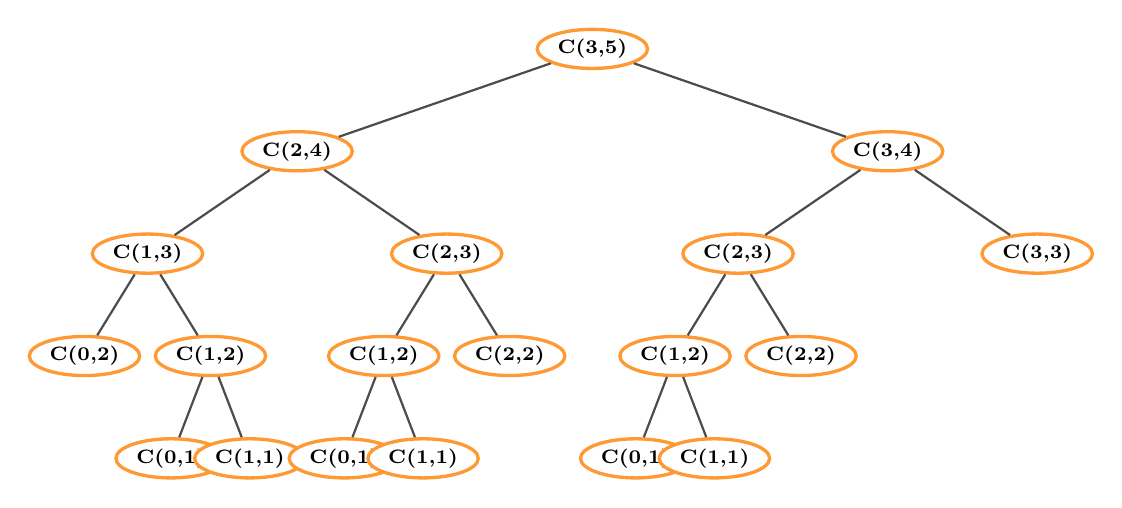
\begin{tikzpicture}[
                    level distance=1.3cm, 
                    level 1/.style={sibling distance=7.5cm},
                    level 2/.style={sibling distance=3.8cm},
                    level 3/.style={sibling distance=1.6cm},
                    level 4/.style={sibling distance=1.0cm}, 
                    node style/.style={
                        ellipse,
                        draw=orange!80,
                        very thick, 
                        fill=white, 
                        align=center, 
                        font=\bfseries\scriptsize, 
                        inner sep=1.5pt,
                        minimum width=1.0cm
                    },
                    edge from parent/.style={draw, thick, black!70}
                ]
                    \node[node style] {C(3,5)}
                        child { node[node style] {C(2,4)}
                            child { node[node style] {C(1,3)}
                                child { node[node style] {C(0,2)} }
                                child { node[node style] {C(1,2)}
                                    child { node[node style] {C(0,1)} }
                                    child { node[node style] {C(1,1)} }
                                }
                            }
                            child { node[node style] {C(2,3)}
                                child { node[node style] {C(1,2)}
                                    child { node[node style] {C(0,1)} }
                                    child { node[node style] {C(1,1)} }
                                }
                                child { node[node style] {C(2,2)} }
                            }
                        }
                        child { node[node style] {C(3,4)}
                            child { node[node style] {C(2,3)}
                                child { node[node style] {C(1,2)}
                                    child { node[node style] {C(0,1)} }
                                    child { node[node style] {C(1,1)} }
                                }
                                child { node[node style] {C(2,2)} }
                            }
                            child { node[node style] {C(3,3)} }
                        };
                \end{tikzpicture}
                }
            \end{center}
        \end{column}
    \end{columns}
\end{frame}

% --- SLIDE 22: ĐỆ QUY CÓ NHỚ – GIẢI PHÁP (TEXT + CODE + CÂY TIKZ) ---
\begin{frame}[fragile]{BÀI TOÁN TÍNH HẰNG SỐ TỔ HỢP – ĐỆ QUY CÓ NHỚ}
    \begin{columns}[T]
        % Cột trái: Lý thuyết giải pháp
        \begin{column}{0.45\textwidth}
            \small
            \begin{itemize}[label=$\bullet$, itemsep=1.0em]
                \item Khắc phục tình trạng một chương trình con với tham số xác định được gọi đệ quy nhiều lần.
                \item Sử dụng bộ nhớ để lưu trữ kết quả của một chương trình con với tham số xác định.
                \item Bộ nhớ được khởi tạo với giá trị đặc biệt để ghi nhận mỗi chương trình con chưa được gọi lần nào.
                \item Địa chỉ bộ nhớ sẽ được ánh xạ với các giá trị tham số của chương trình con.
            \end{itemize}
        \end{column}

        % Cột phải: Code minh họa + Cây đệ quy (Minh họa trùng lặp)
        \begin{column}{0.55\textwidth}
            % 1. Code đệ quy chưa tối ưu (Minted Box)
            \begin{tcblisting}{
                colback=white, colframe=black, boxrule=0.55pt, arc=0pt,
                listing engine=minted, minted language=c,
                minted options={fontsize=\scriptsize, autogobble, baselinestretch=1, style=colorful},
                listing only
            }
int C(int k, int n){
 if (k == 0 || k == n) return 1;
 return C(k-1, n-1)+C(k, n-1);
}
            \end{tcblisting}
            
            \vspace{-0.2cm}
            
            % 2. Cây đệ quy minh họa trùng lặp (Copy từ Slide 21)
            % Dùng resizebox để tự co nhỏ vừa khít phần trống còn lại
            \begin{center}
                \resizebox{0.9\textwidth}{!}{
                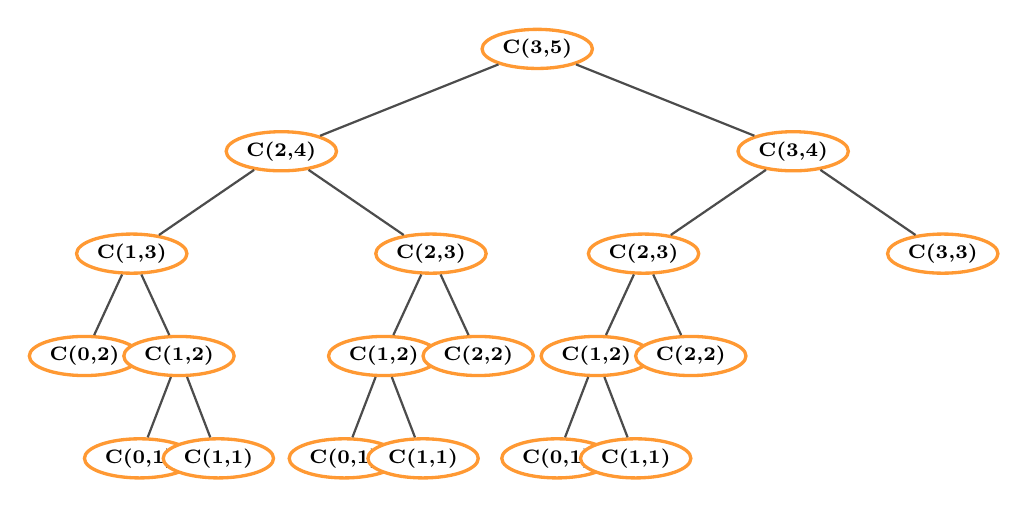
\begin{tikzpicture}[
                    level distance=1.3cm, 
                    level 1/.style={sibling distance=6.5cm},
                    level 2/.style={sibling distance=3.8cm},
                    level 3/.style={sibling distance=1.2cm},
                    level 4/.style={sibling distance=1.0cm}, 
                    node style/.style={
                        ellipse,
                        draw=orange!80,
                        very thick, 
                        fill=white, 
                        align=center, 
                        font=\bfseries\scriptsize, 
                        inner sep=1.5pt,
                        minimum width=1.0cm
                    },
                    edge from parent/.style={draw, thick, black!70}
                ]
                    \node[node style] {C(3,5)}
                        child { node[node style] {C(2,4)}
                            child { node[node style] {C(1,3)}
                                child { node[node style] {C(0,2)} }
                                child { node[node style] {C(1,2)}
                                    child { node[node style] {C(0,1)} }
                                    child { node[node style] {C(1,1)} }
                                }
                            }
                            child { node[node style] {C(2,3)}
                                child { node[node style] {C(1,2)}
                                    child { node[node style] {C(0,1)} }
                                    child { node[node style] {C(1,1)} }
                                }
                                child { node[node style] {C(2,2)} }
                            }
                        }
                        child { node[node style] {C(3,4)}
                            child { node[node style] {C(2,3)}
                                child { node[node style] {C(1,2)}
                                    child { node[node style] {C(0,1)} }
                                    child { node[node style] {C(1,1)} }
                                }
                                child { node[node style] {C(2,2)} }
                            }
                            child { node[node style] {C(3,3)} }
                        };
                \end{tikzpicture}
                }
            \end{center}
        \end{column}
    \end{columns}
\end{frame}

% --- SLIDE 23: ĐỆ QUY CÓ NHỚ – MÃ GIẢ (FIXED MINTED) ---
\begin{frame}[fragile]{BÀI TOÁN TÍNH HẰNG SỐ TỔ HỢP – ĐỆ QUY CÓ NHỚ (MÃ GIẢ)}
    \begin{columns}[T]
        % Cột trái: Text giải thích
        \begin{column}{0.45\textwidth}
            \small
            \begin{itemize}[label=$\bullet$, itemsep=0.8em]
                \item Khắc phục tình trạng một chương trình con với tham số xác định được gọi đệ quy nhiều lần.
                \item Sử dụng bộ nhớ để lưu trữ kết quả của một chương trình con với tham số xác định.
                \item Bộ nhớ được khởi tạo với giá trị đặc biệt (ví dụ 0) để ghi nhận mỗi chương trình con chưa được gọi lần nào.
                \item Địa chỉ bộ nhớ sẽ được ánh xạ với các giá trị tham số của chương trình con.
            \end{itemize}
        \end{column}

        % Cột phải: Mã giả (Box code)
        \begin{column}{0.55\textwidth}
            \begin{tcblisting}{
                colback=white, colframe=black, boxrule=0.5pt, arc=0pt,
                listing engine=minted, minted language=c,
                minted options={fontsize=\scriptsize, autogobble, baselinestretch=1, style=colorful},
                listing only
            }
M[N,N] = {0}; // Initialize 0-array as a memory
              // M[k,n] stores the value C(k,n)
C(k, n){
   if (k == 0 || k == n) M[k,n] = 1;
   else {
      if M[k,n] = 0 then {
         M[k,n] = C(k-1,n-1) + C(k,n-1);
      }
   }
   return M[k,n];
}
            \end{tcblisting}
        \end{column}
    \end{columns}
\end{frame}

% --- SLIDE 24: ĐỆ QUY CÓ NHỚ – CODE HOÀN CHỈNH (FIXED MINTED) ---
\begin{frame}[fragile]{BÀI TOÁN TÍNH HẰNG SỐ TỔ HỢP – ĐỆ QUY CÓ NHỚ (CODE HOÀN CHỈNH)}
    \begin{columns}[T]
        % Cột trái: Text giải thích (Lặp lại để nhắc nhớ)
        \begin{column}{0.45\textwidth}
            \small
            \begin{itemize}[label=$\bullet$, itemsep=0.8em]
                \item Khắc phục tình trạng một chương trình con với tham số xác định được gọi đệ quy nhiều lần.
                \item Sử dụng bộ nhớ để lưu trữ kết quả của một chương trình con với tham số xác định.
                \item Bộ nhớ được khởi tạo với giá trị đặc biệt (ví dụ 0) để ghi nhận mỗi chương trình con chưa được gọi lần nào.
                \item Địa chỉ bộ nhớ sẽ được ánh xạ với các giá trị tham số của chương trình con.
            \end{itemize}
        \end{column}

        % Cột phải: Code C hoàn chỉnh
        \begin{column}{0.55\textwidth}
            \begin{tcblisting}{
                colback=white, colframe=black, boxrule=0.5pt, arc=0pt,
                listing engine=minted, minted language=c,
                minted options={
                    fontsize=\scriptsize, 
                    breaklines,
                    autogobble, 
                    baselinestretch=1, 
                    style=colorful,
                    tabsize=4
                },
                listing only
            }
#include <stdio.h>
#define P 1000000007
#define N 1000
int M[N][N] ={0};

int C(int k, int n){
    if(k == 0 || k == n) M[k][n] = 1;
    else{
        if(M[k][n] == 0){
            M[k][n] = (C(k-1,n-1) + C(k,n-1))%P;
        }
    }
    return M[k][n];
}

int main(){
    int k,n; 
    scanf("%d %d",&k,&n); 
    printf("%d",C(k,n));
    return 0;
}
            \end{tcblisting}
        \end{column}
    \end{columns}
\end{frame}


% --- SLIDE 25: THANK YOU (STYLE SECTION SLIDE) ---
{
\HUSTUseBackground{theme_hust_oneside.pdf}
\begin{frame}
    \placecontent{0.38\paperwidth}{0.45\paperheight}{0.6\paperwidth}{
        \centering
        \color{HUSTRed}\bfseries\fontsize{24pt}{28pt}\selectfont
        THANK YOU!
    }
\end{frame}
}

\end{document}

